%%
%% This is file `sample-sigconf-xelatex.tex',
%% generated with the docstrip utility.
%%
%% The original source files were:
%%
%% samples.dtx  (with options: `all,proceedings,bibtex,sigconf')
%% 
%% IMPORTANT NOTICE:
%% 
%% For the copyright see the source file.
%% 
%% Any modified versions of this file must be renamed
%% with new filenames distinct from sample-sigconf-xelatex.tex.
%% 
%% For distribution of the original source see the terms
%% for copying and modification in the file samples.dtx.
%% 
%% This generated file may be distributed as long as the
%% original source files, as listed above, are part of the
%% same distribution. (The sources need not necessarily be
%% in the same archive or directory.)
%%
%%
%% Commands for TeXCount
%TC:macro \cite [option:text,text]
%TC:macro \citep [option:text,text]
%TC:macro \citet [option:text,text]
%TC:envir table 0 1
%TC:envir table* 0 1
%TC:envir tabular [ignore] word
%TC:envir displaymath 0 word
%TC:envir math 0 word
%TC:envir comment 0 0
%%
%%
%% The first command in your LaTeX source must be the \documentclass
%% command.
%%
%% For submission and review of your manuscript please change the
%% command to \documentclass[manuscript, screen, review]{acmart}.
%%
%% When submitting camera ready or to TAPS, please change the command
%% to \documentclass[sigconf]{acmart} or whichever template is required
%% for your publication.
%%
%%
\documentclass[sigconf,authorversion,nonacm,screen]{acmart}
\settopmatter{printfolios=true}

\usepackage{xeCJK}
% 引入 pseudocode 套件(可放在導言區)
\usepackage[linesnumbered,ruled,vlined]{algorithm2e}
% \usepackage{algcompatible}
\usepackage{tikz}
\setCJKmainfont[AutoFakeSlant=.2,BoldFont={Noto Serif CJK TC SemiBold}]{Noto Serif CJK TC}
\setCJKmonofont{Noto Sans Mono CJK TC}
\setCJKsansfont{Noto Sans CJK TC}


%%
%% \BibTeX command to typeset BibTeX logo in the docs
\AtBeginDocument{%
  \providecommand\BibTeX{{%
    Bib\TeX}}}

%% Rights management information.  This information is sent to you
%% when you complete the rights form.  These commands have SAMPLE
%% values in them; it is your responsibility as an author to replace
%% the commands and values with those provided to you when you
%% complete the rights form.
\setcopyright{acmlicensed}
\copyrightyear{2018}
\acmYear{2018}
\acmDOI{XXXXXXX.XXXXXXX}

%% These commands are for a PROCEEDINGS abstract or paper.
\acmConference[Conference acronym 'XX]{Make sure to enter the correct
  conference title from your rights confirmation emai}{June 03--05,
  2018}{Woodstock, NY}
%%
%%  Uncomment \acmBooktitle if the title of the proceedings is different
%%  from ``Proceedings of ...''!
%%
%%\acmBooktitle{Woodstock '18: ACM Symposium on Neural Gaze Detection,
%%  June 03--05, 2018, Woodstock, NY}
% \acmISBN{978-1-4503-XXXX-X/18/06}


%%
%% Submission ID.
%% Use this when submitting an article to a sponsored event. You'll
%% receive a unique submission ID from the organizers
%% of the event, and this ID should be used as the parameter to this command.
%%\acmSubmissionID{123-A56-BU3}

%%
%% For managing citations, it is recommended to use bibliography
%% files in BibTeX format.
%%
%% You can then either use BibTeX with the ACM-Reference-Format style,
%% or BibLaTeX with the acmnumeric or acmauthoryear sytles, that include
%% support for advanced citation of software artefact from the
%% biblatex-software package, also separately available on CTAN.
%%
%% Look at the sample-*-biblatex.tex files for templates showcasing
%% the biblatex styles.
%%

%%
%% The majority of ACM publications use numbered citations and
%% references.  The command \citestyle{authoryear} switches to the
%% "author year" style.
%%
%% If you are preparing content for an event
%% sponsored by ACM SIGGRAPH, you must use the "author year" style of
%% citations and references.
%% Uncommenting
%% the next command will enable that style.
%%\citestyle{acmauthoryear}


%%
%% end of the preamble, start of the body of the document source.
\begin{document}

%%
%% The "title" command has an optional parameter,
%% allowing the author to define a "short title" to be used in page headers.
\title{Parking Space Price Discrimination via Vehicle Location}

%%
%% The "author" command and its associated commands are used to define
%% the authors and their affiliations.
%% Of note is the shared affiliation of the first two authors, and the
%% "authornote" and "authornotemark" commands
%% used to denote shared contribution to the research.

\author{黃柏凱}
\affiliation{%
  \institution{B11902035}
  \city{}
  \state{}
  \country{}
}

\author{張宸瑋}
\affiliation{%
  \institution{B11902078}
  \city{}
  \state{}
  \country{}
}

\author{黃昱凱}
\affiliation{%
  \institution{B11902158}
  \city{}
  \state{}
  \country{}
}


%%
%% By default, the full list of authors will be used in the page
%% headers. Often, this list is too long, and will overlap
%% other information printed in the page headers. This command allows
%% the author to define a more concise list
%% of authors' names for this purpose.
\renewcommand{\shortauthors}{}

%%
%% The abstract is a short summary of the work to be presented in the
%% article.
\begin{abstract}

\quad 在本次\textbf{研究}中,我們完成C-V2X可行性的調查,之後提出一種與車輛交互的演算法,協助車輛選擇偏好的停車位。接著,我們介紹一套基於定位與交互的停車場營運框架,透過 C-V2X 定位技術實現依停車位區隔的差異化訂價,並分析該框架的優勢並提出該框架的不足之處。

本報告中我們組分工如下:
\begin{itemize}
    \item 黃柏凱: 6 Technical Analysis, 7 Economic Analysis, 8 Discussion, 9 Conclusion.
    \item 張宸瑋: 1 Introduction, 4 Parking Space Recommendation Algorithm, 5.4 Correctness, 5.5 Hardware Requirements, 5.6 Software Requirements
    \item 黃昱凱: 2 Related Work, 3 Localization, 5.1 Explanation, 5.2 FSMs, 5.3 Feature, 8.3 Non-C-V2X Vehicles
\end{itemize}

本報告\textbf{並未}有任何重複提交,也\textbf{未包含}本學期之前已完成的工作。我們是專門為了\textbf{智慧型汽車導論}這門課程而製作此項研究。

本報告使用ChatGPT完成以下事項:輔助閱讀論文,潤稿,輔助生成合適Latex語法;使用Copilot輔助提示python matplotlib.pyplot的語法。
\end{abstract}

%%
%% Keywords. The author(s) should pick words that accurately describe
%% the work being presented. Separate the keywords with commas.


% \received{20 February 2007}
% \received[revised]{12 March 2009}
% \received[accepted]{5 June 2009}

%%
%% This command processes the author and affiliation and title
%% information and builds the first part of the formatted document.
\maketitle

\section{Introduction}

\quad 大型停車場中距離目的地(例如商場門口)可能差上幾百公尺,但所有車位都是相同的定價,因此我們覺得應該要根據距離進行差異化訂價。除此之外,現行的停車場中,要偵測車位是否被占用需要使用超音波或者壓力感應這些需要每個車位各一個的裝置,成本不低。而對於智慧車,若有足夠的基礎設施,僅需少量裝置即可定位智慧車停在哪個車位並以此計價。差異化訂價的方式也可以設定為給予智慧車一些優惠,以鼓勵推廣智慧車。




% 這裡示範如何在文章中使用footcite 來引用文獻\footnote{\cite{}},這個命令會在頁尾自動產生一個包含完整文獻資訊的註腳,同時也會在文章末尾的 Reference 區塊中列出該文獻。

% 這裡示範如何在文章中使用citet 來引用文獻,用法:"根據 \citet{} 的研究......",這個命令會在頁尾自動產生一個包含完整文獻資訊的註腳,同時製造「作者[引用編號]」文字型引用效果。

\section{Related Work}

\quad 過去已有諸多研究提出不同的智慧停車方案,涵蓋即時導引、預約機制與動態收費等技術。其中,\citet{kotb2016iparker}在 2016 年提出的 iParker 系統是一套結合動態資源分配(Dynamic Resource Allocation)與即時價格調整(Dynamic Pricing)的智慧停車平台。該系統採用數學模型(混合整數線性規劃,MILP)來最佳化停車空間分配,並支援即時與事先的預約機制,讓駕駛人可根據個人偏好(例如價格、步行距離)選擇最合適的停車位。iParker 並利用即時佔用率調整各停車資源的費率,有效提升整體資源利用率與收益。

然而,iParker 雖然提出了完整的收費與分配邏輯,其系統設計主要依賴使用者主動預約與感測器回報的佔用資訊,未針對車輛實際所停車格的辨識方式進行深入探討。此外,該系統並未納入車聯網技術或高精度定位資訊作為定位來源。

相較之下,本研究提出以 C-V2X(Cellular Vehicle-to-Everything)為核心的定位方法,透過車輛與基站間的通訊,精準判斷車輛實際停放位置,進而實現停車格層級的辨識能力。此技術突破了現有智慧停車系統在「實際車位判定」上的限制,使得系統不需依賴預約或感測器,也能主動辨識車輛停在哪個停車格。基於此特性,本研究設計的差異化收費機制可根據實際車格條件(例如是否為靠近出入口、遮蔽性佳等)進行價格調整,強化收費彈性與資源管理效率。

綜合來看,iParker 著重於收費與分配策略的最佳化,而本研究則在停車位置辨識的精準性與自動化程度上進行創新,兩者在技術路線上互為補充,亦可作為未來整合應用的基礎。

\section{Localization}
\quad 在智慧停車系統中,實現「不同停車格差異化訂價」的首要技術挑戰,即是準確判斷每輛車實際停放的車格位置。傳統基於圖像識別或地磁感測器的方式,雖可達成基本入位偵測,但成本高、維護不易,且在大型或地下停車場中準確度與可擴展性受限。因此,我們選擇採用 C-V2X(Cellular Vehicle-to-Everything)技術,作為車位級(slot-level)定位的核心手段。

\subsection{C-V2X Based Slot-Level Localization}
\quad 在\citet{5gaa2021v2xhap} 報告中,C-V2X 系統具備提供車格等級(sub-meter)定位精度的能力,透過結合 GNSS、RTK、IMU、5G Cellular Network、HD 地圖等多種感測與通訊技術,在地面或地下停車場等遮蔽環境中亦能維持穩定且精確的定位結果。報告中特別指出,自動駕駛與遠端駕駛等應用需達到 0.1–0.5 公尺等級的定位精度,而該技術已具備支援此一需求的能力,亦可應用於如「停車管理」等商業場景,識別車輛實際停放位置。因此,本研究所採用之 C-V2X 定位模組作為車輛與車格對應判斷機制,不僅具備技術可行性,亦已有業界標準化組織支持其應用於停車定位管理場景。

根據 \citet{liu2021highly} 的研究,他們在論文中所提出的高精度 C-V2X 定位架構,透過融合 GNSS、IMU、5G、RTK 及高精地圖等技術,即使在如停車場等遮蔽環境中仍能提供穩定的定位服務。實際案例顯示,在在 320 公尺 × 50 公尺的工業園區停車場部署六座 5G 基站後,能實現能對 44 個停車格進行高精度定位,其 95\% 的誤差落於 ±1.4 公尺內,已符合一般車位定位需求,證明 C-V2X 技術在智慧停車應用中的可行性與高精度。

此一成果顯示,C-V2X 不僅能用於一般車輛導引與交通控制,也能精確地識別車輛停放的具體位置。因此,在本研究中,我們參考其定位實作架構與融合方法,建構出以 C-V2X 為基礎的停車格定位模組,使每一格車位皆可被車端或後端平台精準識別。如此,即可根據停車格的地點(如靠近出入口、陰影區、充電樁旁等)、停車需求或其他使用情境設計不同價格,實現智慧化與個性化的停車費率策略。

這篇論文提供的實證與架構驗證了我們的技術選擇是具可行性且具備產業應用前例的,亦為我們後續推動基於位置差異化收費的設計奠定了基礎。

\subsection{Comparison between Localization Methods}

\quad 為了準確判斷車輛停在哪個停車格,本研究比較了幾種常見的車輛定位技術,評估其精度、成本、適用場域與部署難易度。以下是各種定位技術的優缺點整理,以及為何 C-V2X 是現階段最合適的選擇。

\begin{table}[h]
\centering
\begin{tabular}{|p{2.5cm}|p{3cm}|p{2.5cm}|}
\hline
\textbf{技術} & \textbf{優點} & \textbf{缺點} \\
\hline
GPS & 廣泛支援,室外表現良好 & 地下室無法使用;難以防止車輛偽造位置  \\
\hline
Camera-based & 精度高,可結合車牌辨識 & 成本高,每個停車位皆需要一個設備;受光影與天氣因素干擾;隱私問題  \\
\hline
Bluetooth Beacon & 成本低,易部署 & 精度差,易受干擾   \\
\hline
UWB (Ultra Wideband) & 精度極高,抗干擾能力強 & 設備昂貴,需標定 \\
\hline
Wi-Fi RTT (Round Trip Time) & 利用現有 Wi-Fi AP 可降低成本 & 需支援 RTT 協定,誤差波動大 \\
\hline
RFID & 成本低;可識別車輛進出 & 無法精準定位格位 \\
\hline
C-V2X & 室內外皆可用;除了定位還能與車輛通訊;成本低,只需要少量基站,且基站可以與5G基站共用 & 初期需設備支援與基地台部署  \\
\hline
\end{tabular}
\caption{各種車輛定位技術比較}
\end{table}

綜合考量,C-V2X 在精度、室內外適應性與部署成本上,具有明顯優勢。其高精度定位與低部署密度的特性,使其成為辨識車輛所在格位的最適解。此外,C-V2X 易於與智慧交通系統整合,具備未來擴展性,因此,我們將假設本作之後的定位系統使用C-V2X實作。

% 綜上所述,C-V2X 在精度、成本與可用性之間取得良好平衡,是實作智慧停車格定位的理想方案。

\section{Parking Space Recommendation Algorithm}

\subsection{Explanation}

\quad 我們提出了一個根據駕駛的偏好,用於幫助駕駛尋找最適合停車位的演算法。此演算法的輸入中,status至少要包含每個停車位是否被使用的資訊,可以額外包含其他資訊(例如位置);pricing function用來決定每個停車位的價格;compare function代表一位駕駛的停車位偏好函式。

此演算法先對所有車位進行分群,將相似的車位分在同一群,交由駕駛決定喜歡哪個車位,然後將此群再次分為更小的數個群,重複這樣的分群-比較行為,直到一個群中的停車位數量足夠少,最終比較此群中的所有停車位,以此決定最適合的停車位。

\subsection{Pseudo Code}
\hyperref[ag:best]{Algorithm 1}與\hyperref[ag:sub]{Algorithm 2} 是我們提出的停車位推薦演算法,其中Algorithm 2中的functions可以根據需求自行調整實作方式。

% 以下為演算法的 pseudocode
\begin{algorithm}[h]
\caption{停車場最佳停車位選擇演算法}
\label{ag:best}

\KwIn{\\
\quad $status$: The state variable of the parking lot indicates the occupancy of each parking space and other informations\;
\quad $pricing(\cdot)$: The algorithm to decide the price of a parking space given its status\;
\quad $compare(\cdot,\cdot)$: The function to compare the which of two parking spaces is better for the agent entering the parking lot\;
\quad $C$: The minimum cluster size threshold to stop clustering\;
}
\KwOut{The best parking space for the agent($bestSpot$)}

\BlankLine
\SetAlgoLined

% 1. 偵測到車輛進入停車場

\For{$i \leftarrow 1$ \KwTo $size(status)$} {
    $status[i].\text{add}(pricing(status[i]))$\;
}

% 2. 根據當前狀態,建立初步集群
$clusters \leftarrow \text{GenerateInitialClusters}(status)$\;%\tcc*{將車位依位置、定價劃分為多個集群}

% 3. Agent 在初步集群中挑選一個集群
$selected \leftarrow \text{SelectCluster}(clusters,\,compare)$\;

% 4. 若選中的集群尚未細分到「常數定義的最小單位」則繼續細分
\While{$size(selected) > C$}{
    $subClusters \leftarrow \text{SubdivideCluster}(selected)$\;
    % \tcc*{將當前集群再細分成子集群}
    $selected \leftarrow \text{SelectCluster}(subClusters,\,compare)$\;
}

% 5. 進入最細分的集群後,列出所有可用車位
$candidateSpots \leftarrow \text{ListAvailableSpots}(selected)$\;

% 6. 依照 compare 排序,選出最優車位
$sortedSpots \leftarrow \text{Sort}(candidateSpots,\,compare)$\;
$bestSpot \leftarrow \text{First}(sortedSpots)$\;

\Return{$bestSpot$}\;
\end{algorithm}

\newpage

\begin{algorithm}[b]
\caption{停車場最佳停車位選擇演算法子程序}
\label{ag:sub}
% 以下為各子程序說明(可視需要實作或當作黑盒處理)
\BlankLine
\SetAlgoLined

\SetKwFunction{FGenInit}{GenerateInitialClusters}
\SetKwProg{Fn}{Function}{}{end}
\Fn{\FGenInit{$status$}}{
    % 依據停車場 layout 與定價策略,把車位分為幾個初步集群
    % \dots 實作細節
    \tcp*[h]{Divide parking spaces into several preliminary clusters based on parking lot layout and pricing strategy}\\
    \Return{$clusters$}
}
\BlankLine
\SetKwFunction{FAgentSel}{SelectCluster}
\Fn{\FAgentSel{$clusters$, $compare$}}{
    % Agent 遍歷 clusters 內每個代表點,利用 compare 比較各集群的預估「最佳車位」
    % 選擇最符合需求的集群
    % \dots 實作細節
    \tcp*[h]{Let the agent compare each cluster from each representative point in the clusters and select the cluster that best meets the needs}\\
    \Return{$selected$}
}
\BlankLine
\SetKwFunction{FSub}{SubdivideCluster}
\Fn{\FSub{$cluster$}}{
    % 將 cluster 中的車位依更細粒度(如區域、步行距離、定價)再細分成子集群
    % \dots 實作細節
    \tcp*[h]{Divide all parking spaces in the cluster into subclusters and return}\\
    \Return{$subClusters$}
}
\BlankLine
\SetKwFunction{FListSpots}{ListAvailableSpots}
\Fn{\FListSpots{$cluster$}}{
    % 列出 cluster 中所有尚未被佔用的車位
    % \dots 實作細節
    \tcp*[h]{Return all available parking spaces in the cluster, for example:}\\
    $candidateSpots \leftarrow \text{EmptyList}$\;
    \For{$i\leftarrow 1$ \KwTo $size(cluster)$} {
        \If{$status[cluster[i]]$ \text{is Empty}} {
            $candidateSpots.\text{append}(cluster[i])$\;
        }
    }
    \Return{$candidateSpots$}
}
\BlankLine
\SetKwFunction{FSort}{Sort}
\Fn{\FSort{$spots$, $compare$}}{
    % 根據 compare 對所有可用車位進行排序,回傳排序後的列表
    % \dots 實作細節
    \tcp*[h]{Sort the parking spaces by comparison function (preference), the best parking space will be the first}\\
    \Return{$sortedSpots$}
}
\BlankLine
\end{algorithm}

\subsection{Feature}

\begin{itemize}
    \item status可以包含每個停車位各種會影響到駕駛喜好的資訊,例如位置、停車格大小、陰影遮蔽度、夜間照明狀況、是否有充電設施、是否為無障礙車位等,以提供這些資訊來讓駕駛比較車位。
    \item 駕駛反饋可以是由駕駛設定的一個策略自動執行,也可以是真的和駕駛來回交互,此演算法使用clustering即是考慮到人類無法進行上千次停車位之間的比較。
    \item 分群演算法、要分多少群以及分群多少次、可以由停車場方自行決定。
    \item 我方建議駕駛參與前應該要先把價格計算完畢,之後就不能再更改,以免惡意利用駕駛需求謀利,以示公平。同時,停車場應該要在網站等公眾能看見的地方公開實時的車位價格變化,讓所有人都能查到,這可以確保停車場不會利用駕駛偏好惡意謀利,同時也方便尚未抵達停車場的駕駛提前查看。
\end{itemize}

\subsection{Correctness}

\quad 此演算法建立在以下假設之上:
\begin{enumerate}
    \item 駕駛對於停車位的偏好(比較函式)符合total ordering(全序關係)和transitivity(遞移律)。
    \item 分群演算法的輸出中,每個群裡的所有車位足夠相似,且每個群之間的車位整體差別足夠大,並且能夠在一個群之中選出一個代表性車位。此足夠的程度會根據分群次數而逐漸嚴格,且每次分群後一個群的停車位數量必會減少。
    \item $C \geq 1$: 每個群最少必須有一個停車位。
\end{enumerate}

此演算法的核心思想是是根據駕駛的喜好將所有停車位進行排序,提供最適合的車位給駕駛。

由於停車位是依照相似度分群,駕駛對數個群中代表性車位的比較即可取代對於這些群中所有車位的比較,在大幅減少比較時間的同時效果並不會比一個一個比較來得差。

\subsection{Hardware Requirements}

\begin{itemize}
    \item 與C-V2X車輛通訊的設備/基礎設施,且透過此方式可以與駕駛溝通(實時溝通或者駕駛事先設定偏好)
    \item (Optional)收集車位當前狀態資訊的設備
\end{itemize}

\subsection{Software Requirements}

\begin{itemize}
    \item 停車位訂價系統/演算法
    \item 停車位分群演算法
\end{itemize}

\section{Framework of Automatic Parking Lot Operating System}

\subsection{Explanation}
\quad 擁有推薦演算法後,我們便可以使用普通進出場管理設備(閘門、車牌辨識或票卡)與C-V2X通訊設備完成以下經營內容,在這個部分,我們將系統分成三個獨立的FSM,分別代表:進場管理(柵欄),中控系統(通訊基站),出場管理(柵欄),而收費系統可以直接使用現成的任意收費系統,故本作不以描述。

進場閘需要在偵測到車輛後取得車輛的車牌號碼,取得後開啟閘門讓車輛進入,在車輛進入後關閉閘門並繼續等待下一輛車的入場,如此反覆。

在中控系統偵測到車輛入場後,首先確認車輛是否擁有C-V2X的功能,若無則忽略此輛車,使用無C-V2X車輛的方式進行計費(固定價格);若有,給出目前不同區域的各項參數(價格,地點等等),讓駕駛回傳偏好,將駕駛偏好的區域再劃分成小區域回傳,直到駕駛停妥為止。

出場閘偵測到車輛後進行辨識,確認是否付款,當付款後便放行等待下一輛車入場。

\subsection{FSMs}
\begin{figure}[htbp]
\centering
% 入口閘門流程圖
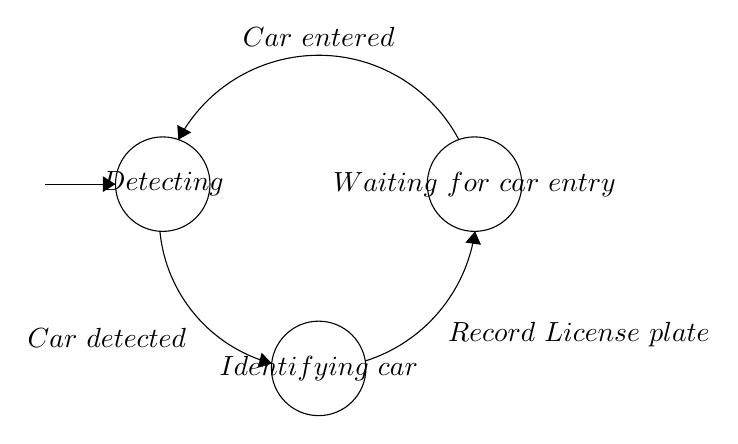
\begin{tikzpicture}[scale=0.2]
\tikzstyle{every node}+=[inner sep=0pt]
\draw [black] (25.5,-29.8) circle (3);
\draw (25.5,-29.8) node {$Detecting$};
\draw [black] (45.3,-29.8) circle (3);
\draw (45.3,-29.8) node {$Waiting\mbox{ }for\mbox{ }car\mbox{ }entry$};
\draw [black] (35.4,-41.5) circle (3);
\draw (35.4,-41.5) node {$Identifying\mbox{ }car$};
\draw [black] (26.492,-26.98) arc (152.08987:27.91013:10.08);
\fill [black] (26.49,-26.98) -- (27.31,-26.51) -- (26.42,-26.04);
\draw (35.4,-21.12) node [above] {$Car\mbox{ }entered$};
\draw [black] (18,-29.8) -- (22.5,-29.8);
\fill [black] (22.5,-29.8) -- (21.7,-29.3) -- (21.7,-30.3);
\draw [black] (32.429,-41.186) arc (-104.9479:-174.57938:9.641);
\fill [black] (32.43,-41.19) -- (31.78,-40.5) -- (31.53,-41.46);
\draw (27.01,-39.54) node [left] {$Car\mbox{ }detected$};
\draw [black] (45.328,-32.789) arc (-7.96822:-72.5045:10.113);
\fill [black] (45.33,-32.79) -- (44.72,-33.51) -- (45.71,-33.65);
\draw (43.58,-39.36) node [right] {$Record\mbox{ }License\mbox{ }plate$};
\end{tikzpicture}
\caption{入口閘門流程圖}
\label{fig:entrance-gate}
\end{figure}



\begin{figure}[htbp]
\centering
% 中控系統流程圖
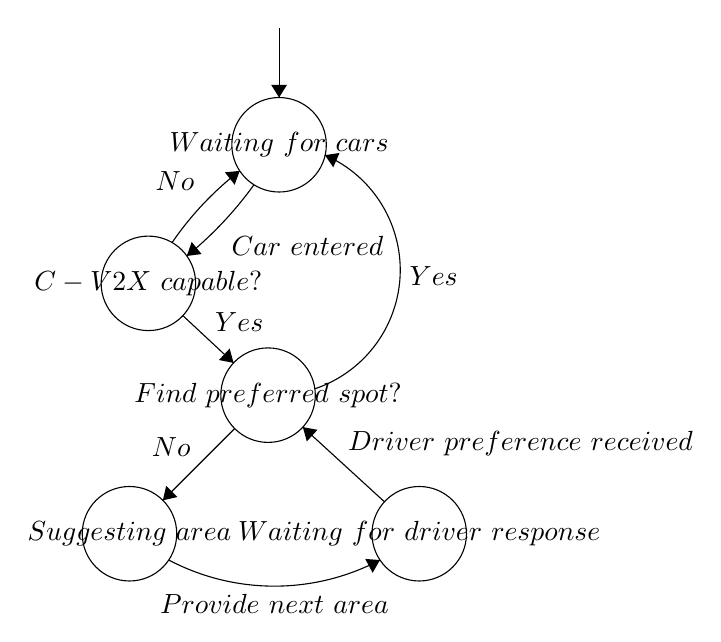
\begin{tikzpicture}[scale=0.2]
\tikzstyle{every node}+=[inner sep=0pt]
\draw [black] (32.5,-18) circle (3);
\draw (32.5,-18) node {$Waiting\mbox{ }for\mbox{ }cars$};
\draw [black] (24.2,-26.8) circle (3);
\draw (24.2,-26.8) node {$C-V2X\mbox{ }capable?$};
\draw [black] (31.8,-33.9) circle (3);
\draw (31.8,-33.9) node {$Find\mbox{ }preferred\mbox{ }spot?$};
\draw [black] (23,-42.7) circle (3);
\draw (23,-42.7) node {$Suggesting\mbox{ }area$};
\draw [black] (41.4,-42.7) circle (3);
\draw (41.4,-42.7) node {$Waiting\mbox{ }for\mbox{ }driver\mbox{ }response$};
\draw [black] (30.906,-20.539) arc (-35.76029:-50.89003:23.605);
\fill [black] (26.64,-25.06) -- (27.58,-24.94) -- (26.95,-24.17);
\draw (29.45,-24.41) node [right] {$Car\mbox{ }entered$};
\draw [black] (26.39,-28.85) -- (29.61,-31.85);
\fill [black] (29.61,-31.85) -- (29.36,-30.94) -- (28.68,-31.67);
\draw (29.97,-29.87) node [above] {$Yes$};
\draw [black] (25.707,-24.209) arc (145.5707:127.77897:20.238);
\fill [black] (30,-19.66) -- (29.06,-19.75) -- (29.68,-20.54);
\draw (27.15,-20.3) node [left] {$No$};
\draw [black] (29.68,-36.02) -- (25.12,-40.58);
\fill [black] (25.12,-40.58) -- (26.04,-40.37) -- (25.33,-39.66);
\draw (25.65,-37.82) node [above] {$No$};
\draw [black] (38.912,-44.366) arc (-62.17624:-117.82376:14.379);
\fill [black] (38.91,-44.37) -- (37.97,-44.3) -- (38.44,-45.18);
\draw (32.2,-46.53) node [below] {$Provide\mbox{ }next\mbox{ }area$};
\draw [black] (39.19,-40.67) -- (34.01,-35.93);
\fill [black] (34.01,-35.93) -- (34.26,-36.84) -- (34.94,-36.1);
\draw (47.83,-37.81) node [above] {$Driver\mbox{ }preference\mbox{ }received$};
\draw [black] (35.409,-18.656) arc (66.48623:-71.52789:7.958);
\fill [black] (35.41,-18.66) -- (35.94,-19.43) -- (36.34,-18.52);
\draw (40.75,-26.32) node [right] {$Yes$};
\draw [black] (32.5,-10.6) -- (32.5,-15);
\fill [black] (32.5,-15) -- (33,-14.2) -- (32,-14.2);
\end{tikzpicture}
\caption{中控系統流程圖}
\label{fig:control-system}
\end{figure}


\begin{figure}[htbp]
\centering
% 離場閘流程圖
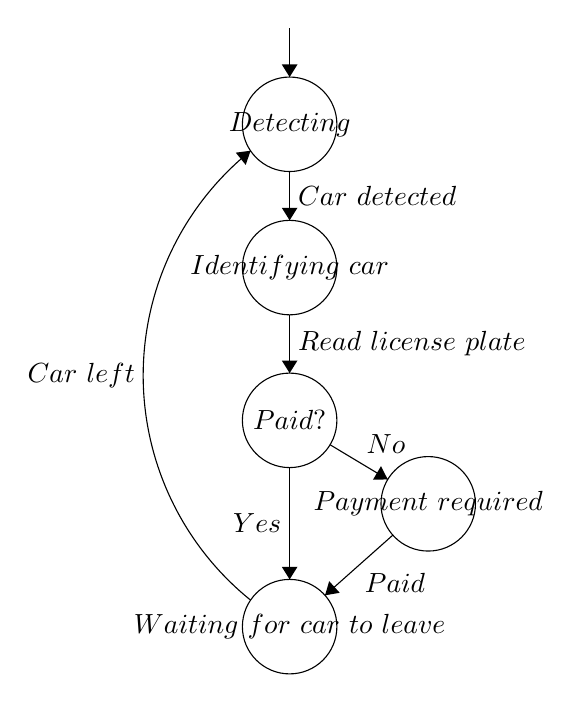
\begin{tikzpicture}[scale=0.2]
\tikzstyle{every node}+=[inner sep=0pt]
\draw [black] (38.5,-6.3) circle (3);
\draw (38.5,-6.3) node {$Detecting$};
\draw [black] (38.5,-15.4) circle (3);
\draw (38.5,-15.4) node {$Identifying\mbox{ }car$};
\draw [black] (47.3,-30.4) circle (3);
\draw (47.3,-30.4) node {$Payment\mbox{ }required$};
\draw [black] (38.5,-25.1) circle (3);
\draw (38.5,-25.1) node {$Paid?$};
\draw [black] (38.5,-38.2) circle (3);
\draw (38.5,-38.2) node {$Waiting\mbox{ }for\mbox{ }car\mbox{ }to\mbox{ }leave$};
\draw [black] (38.5,-9.3) -- (38.5,-12.4);
\fill [black] (38.5,-12.4) -- (39,-11.6) -- (38,-11.6);
\draw (39,-10.85) node [right] {$Car\mbox{ }detected$};
\draw [black] (41.07,-26.65) -- (44.73,-28.85);
\fill [black] (44.73,-28.85) -- (44.3,-28.01) -- (43.79,-28.87);
\draw (44.62,-27.25) node [above] {$No$};
\draw [black] (38.5,-28.1) -- (38.5,-35.2);
\fill [black] (38.5,-35.2) -- (39,-34.4) -- (38,-34.4);
\draw (38,-31.65) node [left] {$Yes$};
\draw [black] (45.05,-32.39) -- (40.75,-36.21);
\fill [black] (40.75,-36.21) -- (41.68,-36.05) -- (41.01,-35.31);
\draw (45.19,-34.79) node [below] {$Paid$};
\draw [black] (38.5,-18.4) -- (38.5,-22.1);
\fill [black] (38.5,-22.1) -- (39,-21.3) -- (38,-21.3);
\draw (39,-20.25) node [right] {$Read\mbox{ }license\mbox{ }plate$};
\draw [black] (36.021,-36.516) arc (-128.88776:-231.11224:18.327);
\fill [black] (36.02,-7.98) -- (35.08,-8.1) -- (35.71,-8.88);
\draw (28.7,-22.25) node [left] {$Car\mbox{ }left$};
\draw [black] (38.5,-0.2) -- (38.5,-3.3);
\fill [black] (38.5,-3.3) -- (39,-2.5) -- (38,-2.5);
\end{tikzpicture}
\caption{出場閘流程圖}
\label{fig:exit-gate}
\end{figure}

\newpage

\subsection{Feature}

\begin{itemize}
    \item 模組化 FSM 架構:系統以三個獨立 FSM(進場管理、計費系統、出場管理)實作,可彈性擴充或針對單一模組調整功能。
\end{itemize}
\begin{itemize}
    \item 自動化進出場流程:整合車牌辨識與 C-V2X 通訊,自動控制柵欄開啟,無須人力或等待時間。
\end{itemize}
\begin{itemize}
    \item 辨識車輛功能:能確認車輛是否擁有C-V2X功能,並依此採用不同策略進行計費等行動。
\end{itemize}
\begin{itemize}
    \item 即時資訊回饋:使用者可透過車載系統或 APP 查詢目前推薦車格、剩餘車位、預估費用等資訊,提升體驗。
\end{itemize}

\subsection{Correctness}

\quad 此演算法建立在以下假設之上:
\begin{enumerate}
    \item 車輛會以正常方式進出停車場,且只會停在一格停車格之內。
    \item 有方法(例如由OEM提供)可以偵測C-V2X是否由車輛發出
    \item C-V2X在停車過程中全程開啟;或者保證啟動車輛時C-V2X必定會跟著啟動且連接到停車場方
\end{enumerate}

第一點是假設駕駛不會惡意停車,例如停在兩個停車格中間;第二點是為了避免人拿著裝有C-V2X的行動裝置偽裝成車輛;第三點是避免駕駛在低價位的停車格停車後再次啟動車輛停到另一價格更高的停車位,因此停車場方必須要有能追蹤車輛正確位置的能力。

只要保證車輛與駕駛行為遵守規則,或者能夠檢測違反規則的行為,即可保證以上FSMs的正確性。

\subsection{Hardware Requirements}

\begin{itemize}
    \item 與C-V2X車輛通訊的設備/基礎設施,同時也是作為偵測車輛是否有C-V2X的方法。
    \item 車牌辨識設備(僅在停車場出入口需要)
\end{itemize}

\subsection{Software Requirements}

\begin{itemize}
    \item 停車位訂價系統
    \item 支付系統
    \item 停車位推薦演算法
\end{itemize}

\section{Technical Analysis}

\quad 我們會相對目前市面上已經成熟的智慧停車場管理系統進行比較,主要針對使用紅外線進行在席車位辨識並以LED導引指示燈為顯示方式的停車導引系統,在功能性與建設成本上探討我們的優勢。當然,正如我們起初設想,我們的架構也可以與現行系統合併使用,與車格的檢測結果交叉驗證,以增加彼此的精度。

\subsection{Advantages of Functionality}

\quad 相較於現行系統,我們能做到:

\begin{enumerate}
    \item 基於時間與空間的動態價格調整
    \item 自動/手動車位推薦
    \item 停車位置查詢
    \item 車位佔用程度查詢
\end{enumerate}

其中基於紅外線的停車導引系統僅能做到第四點,且經常因為設備問題、車輛停放角度問題而失靈,至於基於攝影機的在席車牌辨識,可以再做到第三點,但一二兩點要求與車輛高度交互的能力,若實作於非智慧車/舊系統中,例如在基於攝影機的停車導引系統加入入場QR code供駕駛人為掃描、進入、查看並選擇,將導致入口雍塞或駕駛頻繁分心。

此外,在大型的戶外場景中,鋪設基於車位的攝影機或紅外線感應器不論在成本上還是可靠性上都將面臨巨大的考驗,至於與5G技術同源的C-V2X通訊基站在戶外的使用場景早有充分的可靠性驗證。

\subsection{Advantages of Construction Cost}

\quad 為求簡單並避免一些身份驗證問題,我們假設進場管制中具有車牌辨識系統,在台灣,停車場的車牌辨識普及率相當高,例如根據交通部年鑑,台北市公有停車場已全部安裝車牌辨識系統\footnote{\cite{motc111_taipei_parking}},臺中市公共停車場自111年起也有65.4\%使用車牌辨識系統\footnote{\cite{motc111_taichung_parking}},因此我們暫時不考慮出入口車牌辨識的建設成本。

在這些停車場中,僅需依規模加裝少量C-V2X通訊基站,甚至能與既有的5G通訊基站共用,並且使用一個消費級的計算單元(小型停車場也可嘗試整合進自動繳費機中),就能夠管理面積龐大的停車空間。

最理想情況下,一座有基站控制能力(與電信業者合作)與車牌辨識系統的停車場,可以僅在軟體層面升級的條件下完成整套架構的部署。務實情景中,基站的建設成本也遠低於現行對每個車位的紅外線感應甚至車牌辨識攝影機(如需實作尋車系統)。

\subsection{Advantages of Profit}

\quad 我們將在\hyperref[sec:EA]{下個章節}中對本架構的經濟效益進行詳細討論。


\section{Economic Analysis}
\label{sec:EA}

\quad 在這個章節中,我們將試圖論證我們的架構具有商業模式下的可行性與優越性,我們將相較於傳統商業模型,即固定價格式收費模式,並假設採納本架構的經營者採用我們的建議商業模型,即:

\begin{enumerate}
    \item 不去調漲傳統車輛的費率,並作為智慧車輛的最高費率。
    \item 在尖峰時段(即能停滿的時段)中所有車輛皆保持最高費率。
    \item 在離峰時段中,以車位的吸引力為條件制定智慧車輛的優惠費率。
\end{enumerate}

其中吸引力可以有諸多因素,為求簡化,我們以人員出入口的步行距離為依據調整,並期待該方法貼合消費者的願付價格。實際操作中可以使用機器學習或其他工具計算期望願付價格以最大化經營者的利潤。

至於市場環境,我們為求簡單展示,假設市場被分成尖峰時段與離峰時段兩種需求模式且各佔一半的規模(時間),實際情況中的需求截距(\hyperref[fig:TM]{圖四}與\hyperref[fig:OM]{圖五}的參數a)對時間的分布更可能是一個連續曲線。

我們將使用長期市場作為展示模式,即生產者(停車場經營方)的建設成本將被時間折舊,且資本將自由進出市場。

\subsection{Traditional Model}

\quad 我們先展示一個傳統商業模型下的供需圖(\hyperref[fig:TM]{圖四}):

\begin{figure}[h]
    \centering
    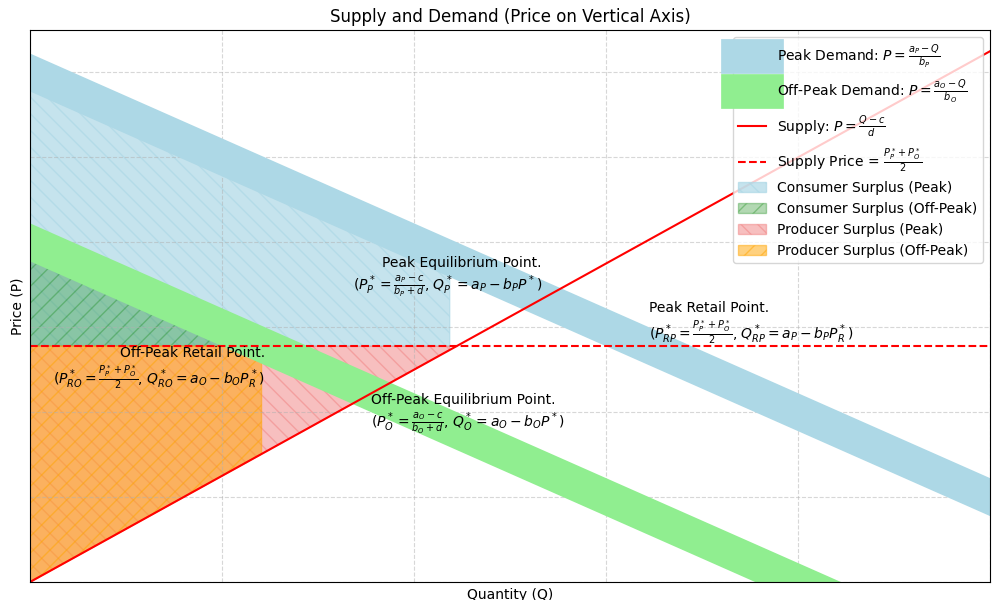
\includegraphics[width=1.0\linewidth]{TM.png}
    \caption{傳統商業模型長期尖峰離峰供需圖}
    \label{fig:TM}
\end{figure}

在該圖中,我們假設價格採尖峰均衡價格與離峰均衡價格的平均(紅虛線),在各佔一半規模的假設下,這是最大化收益的選擇,藍線與綠線的寬度代表不同價值的車位之間的需求差異(互為替代品),其與紅虛線的交點即為尖峰與離峰的銷量,因為我們評估長期供給,所以無需考慮滿位問題,即新停車場將被建設若長期供不應求。

\subsection{Our Model}

\quad 接下來是本作的商業模型的供需圖(\hyperref[fig:OM]{圖五}):

\begin{figure}[h]
    \centering
    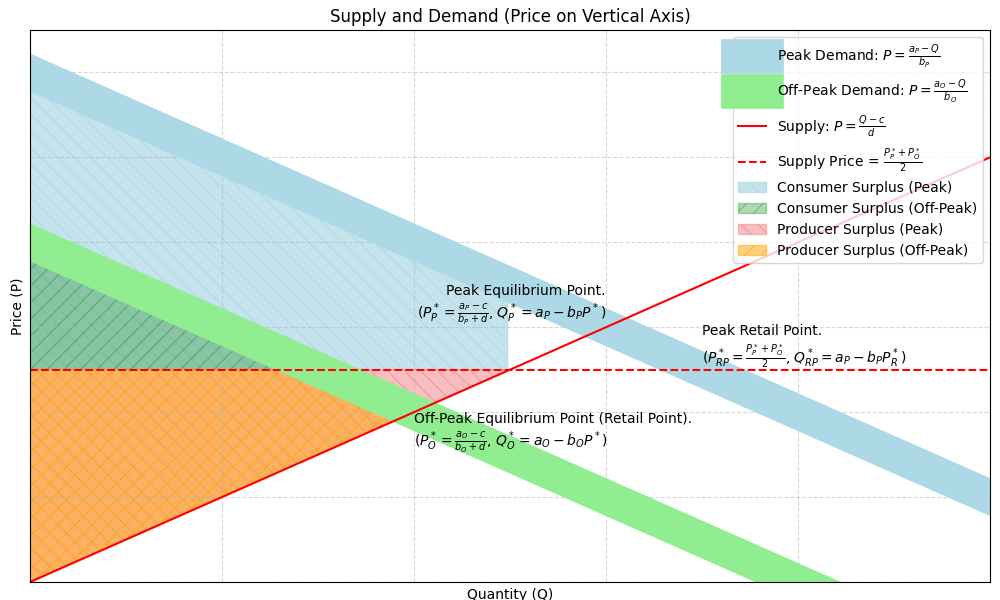
\includegraphics[width=1.0\linewidth]{OM.png}
    \caption{本作商業模型長期尖峰離峰供需圖}
    \label{fig:OM}
\end{figure}

首先,本方案具有更低的建設成本(正比於參數\(d\),反比於紅實線斜率),這直接導致了更大的銷量與更低的售價,即經濟學上的技術革新。

接著有鑒於我們採用共用模式,並假設尖峰時段不特別漲價,因此僅在離峰時段的零售價格回歸均衡價格(對智慧車而言)。此外,訂價不再是以藍綠粗線的均衡點,而是以其跨度所截的供給線段(紅實線)為底,最高價格(紅虛線)為頂,進行差異化訂價。

\subsection{Economic Advantages for Traditional Vehicles}
\label{sec:ET}

\quad 使用傳統車輛的個體消費者亦可享受本方案的技術革新導致的終端零售價格降價(消費者剩餘增加),雖然他們無法使用部份智慧停車場的功能。

\subsection{Economic Advantages for Intellegent Vehicles}

\quad 使用智慧車輛的個體消費者除了\hyperref[sec:ET]{上述}優惠,亦可直接享受離峰時段的價格優惠與基於車格吸引力的價格優惠,在更多C-V2X車主的成熟模式中,擁有更高需求的車主可以使用更高的金額獲得更好的車位,而非傳統的先到先得。

\subsection{Economic Advantages for Parking Lot Operators}

\quad 除了技術革新導致的生產者剩餘增加外,\hyperref[fig:TM]{圖四}中離峰時段的無謂損失在\hyperref[fig:OM]{圖五}中完全由生產者獲得,即使用差異化訂價策略成功使停車場經營者獲得更多的收益。


\subsection{Other Economic Potential}

\quad 假設僅考慮經營方的立場,我們亦可試著將基礎費率調漲,以更加貼合需求的變動。此外,若是僅經營智慧車輛,亦可直接放棄對原先價格上限的假設,實施完全的差異化訂價。

\section{Discussion}

\subsection{Security Chellenge}

\quad 我們在計費實作中,必須假設C-V2X在停車過程中全程開啟,以防止駕駛在低費區段關閉C-V2X後停往高費區段。該問題在長期停車中尤為明顯(油車或許無法承擔以週為單位的通訊電量消耗)。可能的解決方案有指數級增加每個檢查階段間的等待時間或是降低定位階段的精度要求等,也可以藉由制定車輛啟動時C-V2X必須開啟的技術保證標準,來接受僅使用進場/出場前的資訊計價。

此外,本作未提及身份安全性的實作議題,我們希望藉由既有的PKI進行基於車牌為個體的公鑰管理,以進行身份驗證與非對稱加密通訊,但這涉及更多標準的制定,故我們選擇保留此議題。

\subsection{Extensibility}

\quad 本作的停車系統並未考慮除汽車以外的其他機動載具(摩托車、遊覽車等)所對應或混合使用的停車場的技術與商業之可行性,但我們傾向於相信隨智慧型載具的普及使用,本作的架構亦可與他們相容。

此外,隨定位精度技術的提升,我們亦可將此架構應用於以城區為單位進行路邊停車的停車格管理,以將本作的諸多優勢應用於其餘停車空間。

\subsection{Non-C-V2X Vehicles}
\quad 由於包含C-V2X功能的智慧車輛普及化需要一段時間,智慧停車場系統在此過渡期仍需考量非 C-V2X 車輛的進場與管理需求,帶來數項挑戰。停車場無法透過 C-V2X 即時得知車輛的停放位置,也無法藉由 C-V2X 驗證車輛身份,導致無法實施基於車格位置的動態服務與差異化計價策略。

針對上述限制,可考慮以現有的車格偵測技術(紅外線感測)作為過渡性解決方案。雖然此類技術無法提供針對某停車格停放車輛的身份辨識功能,但足以判斷車格的占用狀態。系統可據此排除被非 C-V2X 車輛占用的車位,避免將其推送給具備 C-V2X 功能的車輛,從而確保整體運作的精準度與服務品質。

在計價策略方面,可將無法確認車輛身份的車位,預設為理論上的最高價位,以維護差異化訂價機制的公平性。此舉亦有助於鼓勵駕駛升級或採用具備 C-V2X 功能之車輛,以享有更優惠之停車費率與智能化服務。
\subsection{Special Space Usage}

\quad 本作並未提及特殊停車空間(如身心障礙車位、電動車充電車位等)的實作方式,因為我們認爲現階段基於公民的集體道德共識與智慧地鎖設備等基礎手段已經足夠完整,尚且不需要處理相關問題。不過,基於相同的思路,我們也可以將原先基於車牌辨識的智慧地鎖設備改為基於C-V2X,以在應用差別費率的同時進行特殊車位的管制。

\section{Conclusion}

\quad 我們確認了C-V2X技術使用於車格定位的可行性,並分析C-V2X與其他技術的優劣。我們完成了差異化訂價的使用者交互演算法並驗證其可行性,以期許該演算法可以自動或半自動地接入智慧車輛並完善自動駕駛在停車場的策略。

在驗證交互與定位的可行性後,我們提出了以車輛定位實施智慧停車場與差異化訂價的框架並驗證其可行性,我們分析該框架相較於傳統智慧停車場方案,確定其在技術層面具有功能優勢。隨後我們提出一個商業模式,並使用經濟學分析,證明其相較於傳統智慧停車場方案,對車主與停車場經營方皆有更大的收益,形成雙贏。

在優勢之餘,我們也指出該架構的有限之處與未完成之處,以供後續研究者與標準、協議制定方參考。

%%
%% The next two lines define the bibliography style to be used, and
%% the bibliography file.
\bibliographystyle{ACM-Reference-Format}
\bibliography{reference.bib}

\end{document}
\endinput
%%
%% End of file `sample-sigconf-xelatex.tex'.
